\documentclass{article}
\usepackage{hyperref}
\usepackage{graphicx}
\usepackage{listings}

\title{INFO-F-311: Artificial Intelligence - Project 2: Recherche adversariale}
\author{Bourgeois Noé}
\date{2023 October 29}

\begin{document}

\maketitle

\tableofcontents

\newpage
\section{Introduction}
This report outlines the application of adversarial search techniques in graph search problems. 
For references, please refer to the project instructions and the project 1.

\section{Better evaluation function}
% \section{Differences in \texttt{BetterValueFunction} Compared to \texttt{WorldMDP}}

\subsection{\texttt{get\_available\_actions\_ordered}}
\begin{center}
    \begin{tabular}{|c|c|}
    \hline
    Algorithm & Time Complexity \\
    \hline
    Minimax & \( O(b^m) \) \\
    \hline
    Alpha-Beta & \( O(b^{m/2}) \) to \( O(b^m) \) \\
    \hline
    Alpha-Beta with Perfect Ordering & \( O(bm/2) \) \\
    \hline
    \end{tabular}
    \end{center}
    
    \vspace{1em} % Add some space after the table
    

In the \texttt{BetterValueFunction} class, this method orders the available actions based on certain conditions:

\begin{itemize}
    \item Moves the action \texttt{STAY} to the end of the list.
    \item If not all gems are collected, it prioritizes actions that lead to a gem.
    \item If the agent's path intersects with dangerous lasers, it de-prioritizes such actions.
\end{itemize}

\subsection{Method: \texttt{transition}}
In this method, the value of a state is changed based on multiple factors:
\begin{itemize}
    \item The distance of agents to gems and exit points.
    \item Whether all gems are collected or not.
\end{itemize}

\newpage
\section{Results}
\subsection{Fewer Nodes with Better Evaluation}
\subsubsection{First Map}

\begin{table}[h]
    \centering
    \begin{tabular}{|c|c|c|c|}
    \hline
    . & G & S1 \\
    \hline
    L0E & S0 & .\\
    \hline
    X & @ & X \\
    \hline
    \end{tabular}
    \label{tab:example_grid}
\end{table}

\begin{figure}[h]
    \centering
    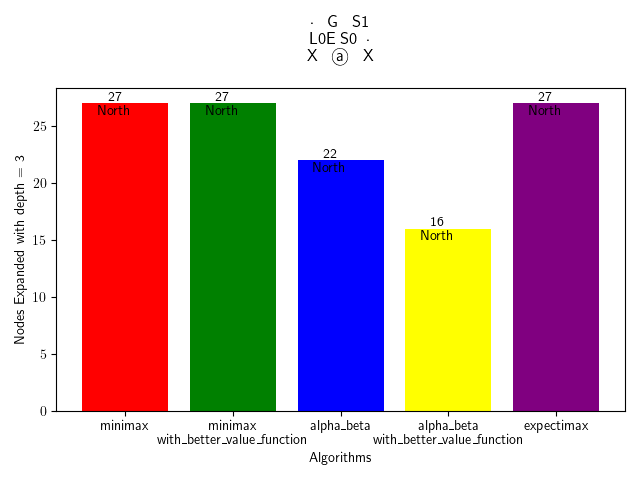
\includegraphics[width=\textwidth]{media/map2023_10_29_13_48_15.png}
    \caption{Map 1}
    \label{fig:image1}
\end{figure}
\vspace{1em}


    
\paragraph{}
Here we can see that, compared to \texttt{alpha\_beta}, 
the number of nodes is reduced by 6. 
Additionally, compared to \texttt{minimax}, 
the number of nodes is reduced by 11. 
This is what we expected, because we have a better evaluation function.

\begin{figure}[h]
    \centering
    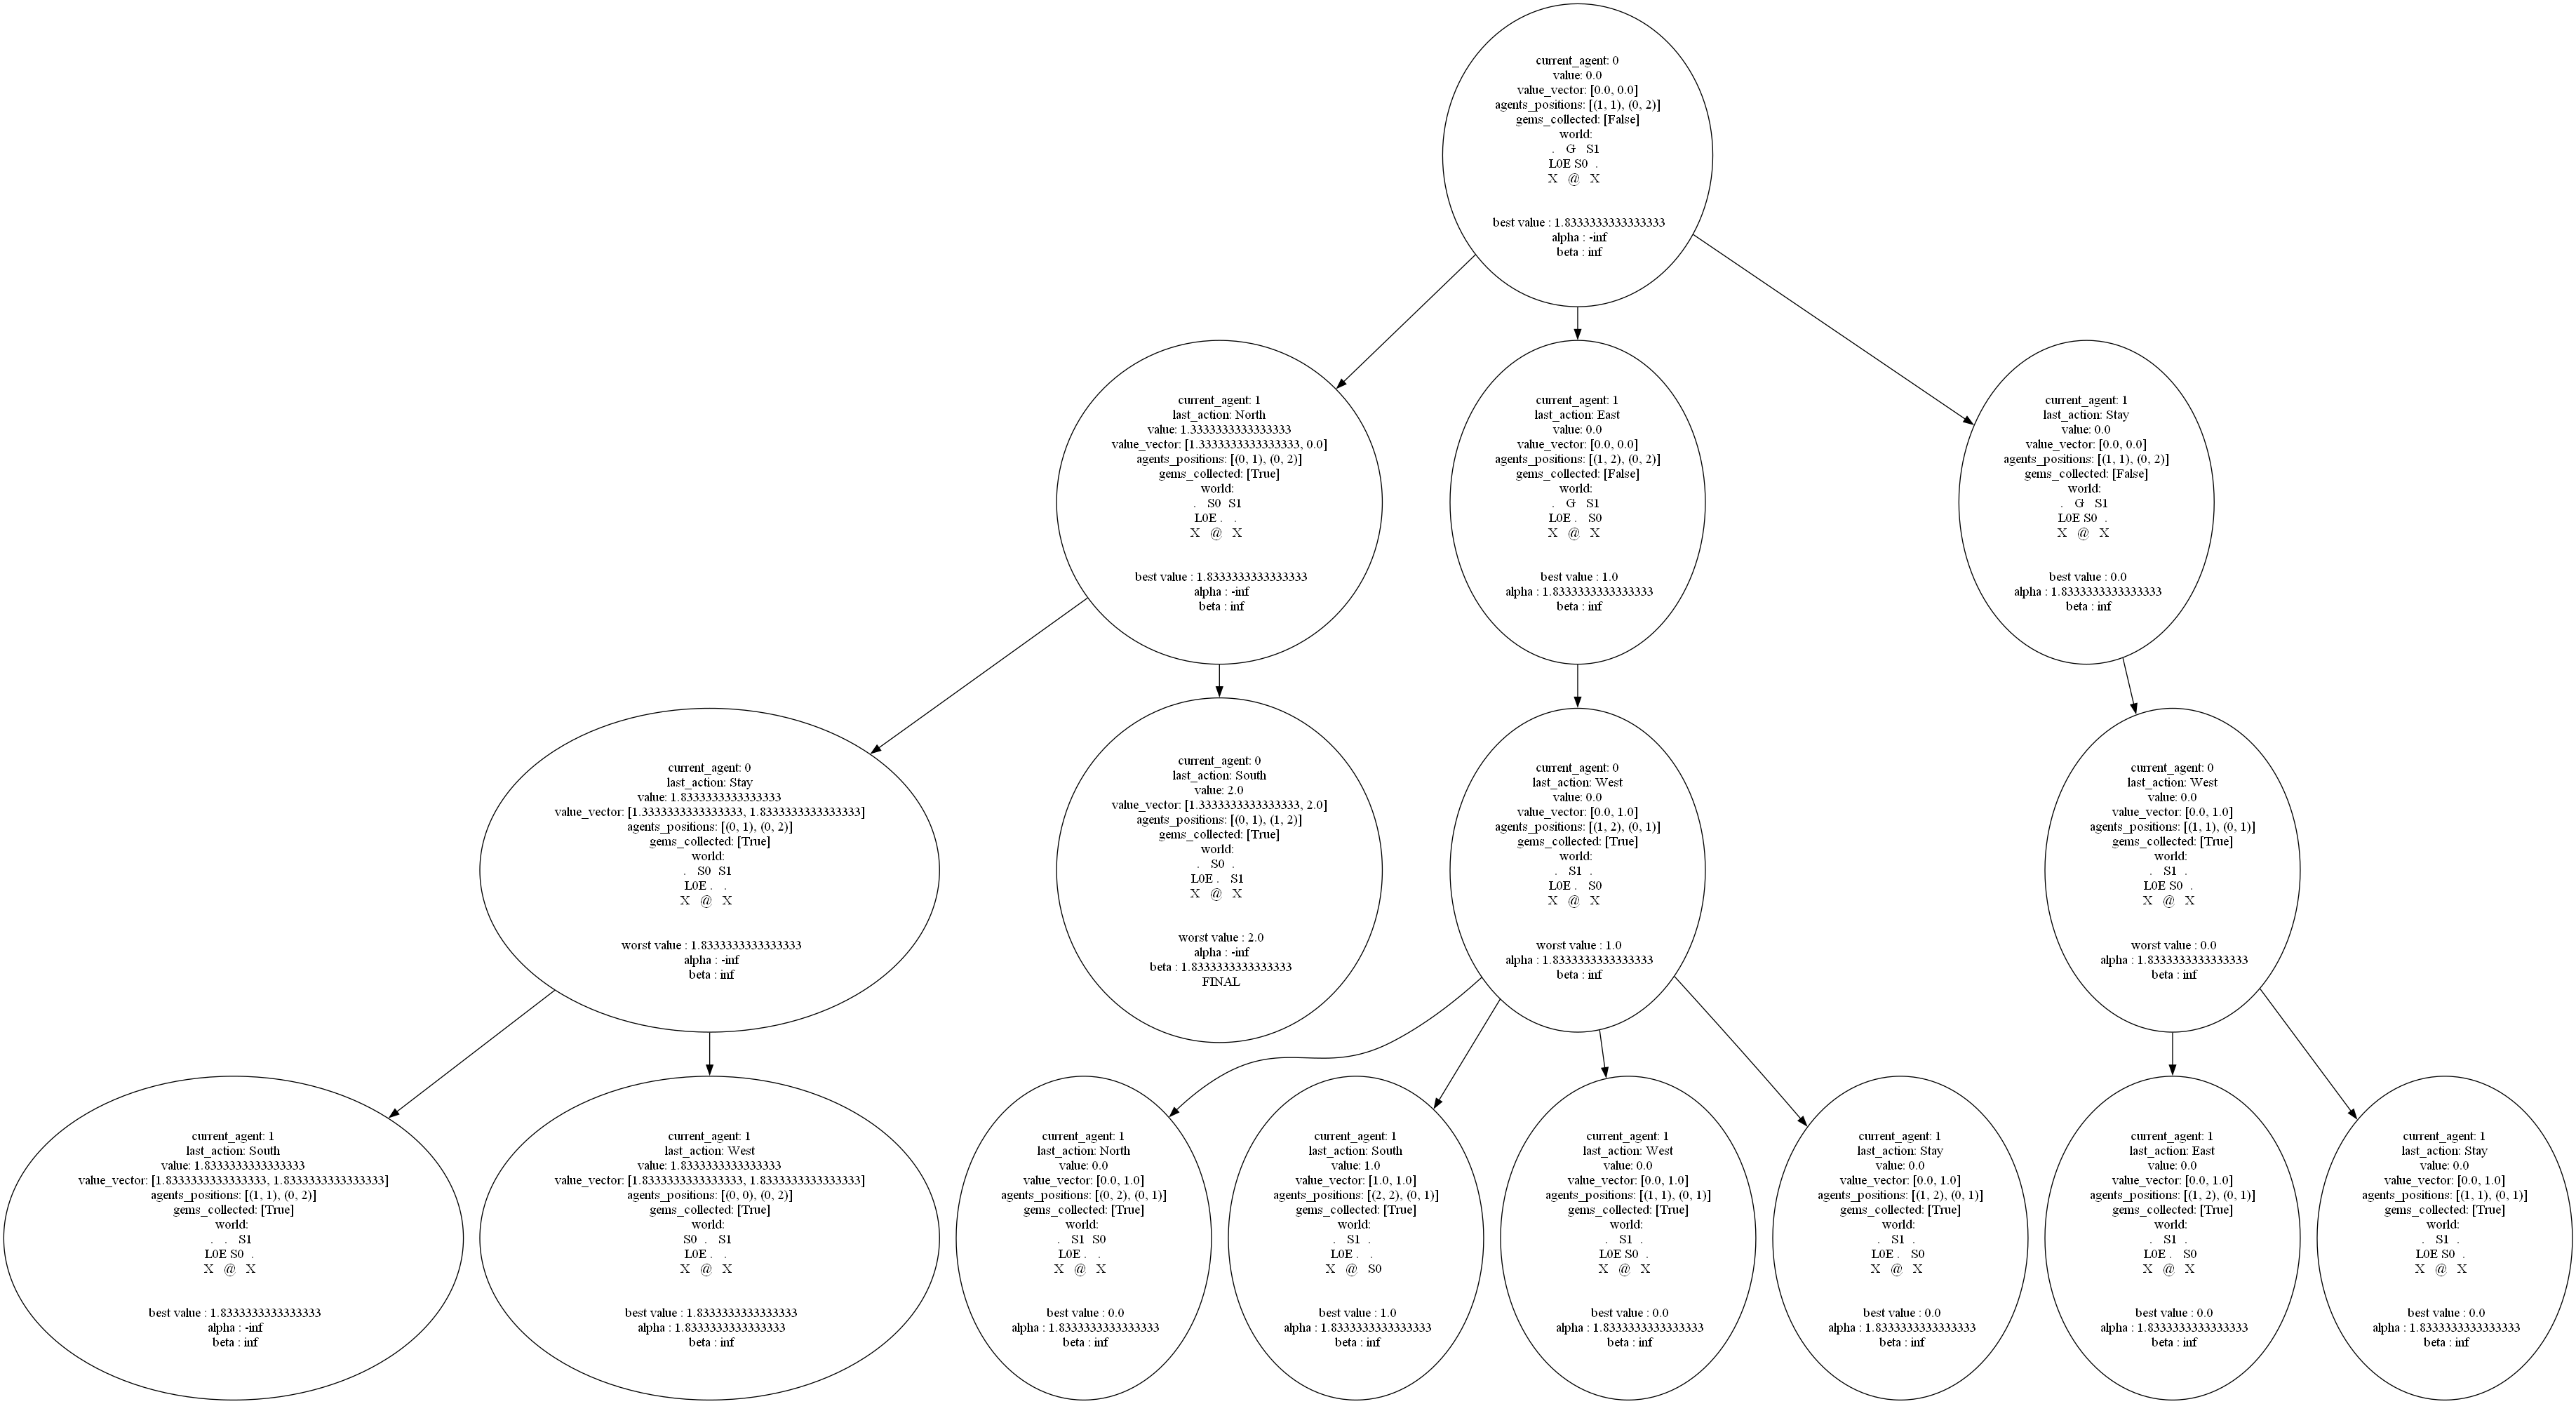
\includegraphics[width=\textwidth]{media/20231029-134819.png}
    \caption{First map's Better Evaluation Markov Decisional Process Tree}
    \label{fig:image1tree}
\end{figure}
\vspace{1em}


\newpage
\newpage
\subsubsection{Second Map}

\begin{table}[h]
    \centering
    \begin{tabular}{|c|c|c|}
    \hline
    . & X & G \\
    \hline
    @ & @ & S0 \\
    \hline
    . & . & . \\
    \hline
    . & . & . \\
    \hline
    . & X & S1 \\
    \hline
    \end{tabular}
    \label{tab:grid}
    \end{table}
    

    
\begin{figure}[h]
    \centering
    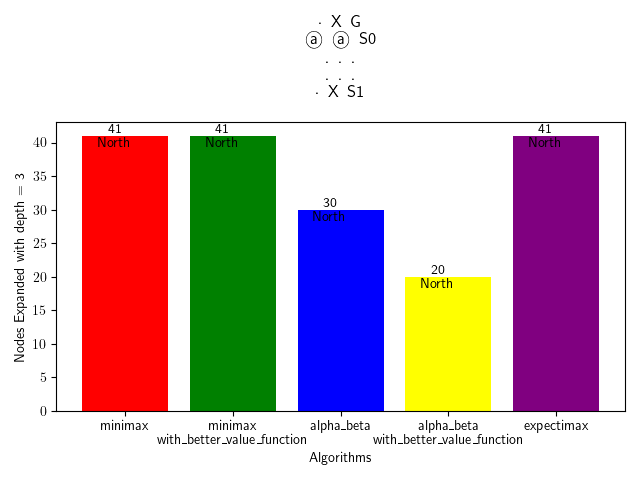
\includegraphics[width=\textwidth]{media/map2023_10_29_13_56_42.png}
    \caption{Map 2}
    \label{fig:image2}
\end{figure}
\vspace{1em}

\paragraph{}
Again, we can see that, compared to \texttt{alpha\_beta},
the number of nodes is reduced and compared to \texttt{minimax},
the number of nodes is reduced by factor 2.


\newpage
\subsubsection{Third Map}

\begin{table}[h]
    \centering
    \begin{tabular}{|c|c|c|c|c|c|}
    \hline
    G & . & . & . & . & G \\
    \hline
    X & . & G & S2 & S0 & G \\
    \hline
    . & . & G & X & S1 & X \\
    \hline
    . & . & G & . & . & . \\
    \hline
    \end{tabular}
    \label{tab:your_grid}
    \end{table}
    
\begin{figure}[h]
    \centering
    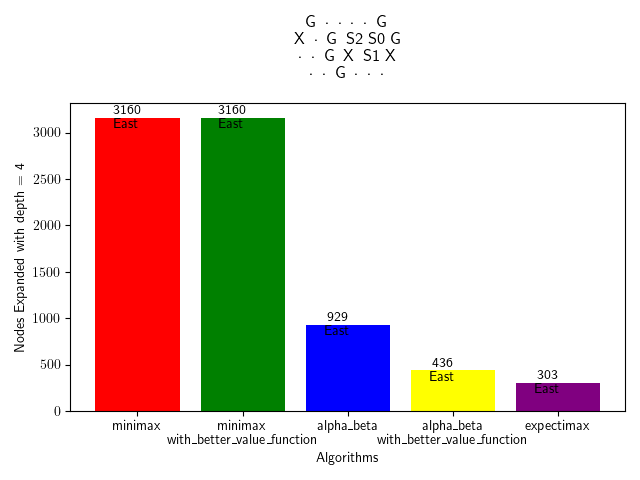
\includegraphics[width=\textwidth]{media/map2023_10_29_13_53_25.png}
    \caption{Map 3}
    \label{fig:image3}
\end{figure}
\vspace{1em}

\paragraph{}
Here again, with a slightly bigger map and whith a much bigger difference with factors of 2 and 7.
It is to note that \texttt{expectimax}, without any heuristic, has the lowest number of nodes, with correct action.


\newpage
\subsection{Fourth Map}

\begin{table}[h]
    \centering
    \begin{tabular}{|c|c|c|c|}
    \hline
    S0 & S2 & X \\
    \hline
     & G & \\
    \hline
    @ & & G \\
    \hline
     & S1 & \\
    \hline
     & X & X \\
    \hline
    \end{tabular}
    \label{tab:another_example_grid}
\end{table}

% Fourth Image
\begin{figure}[h]
    \centering
    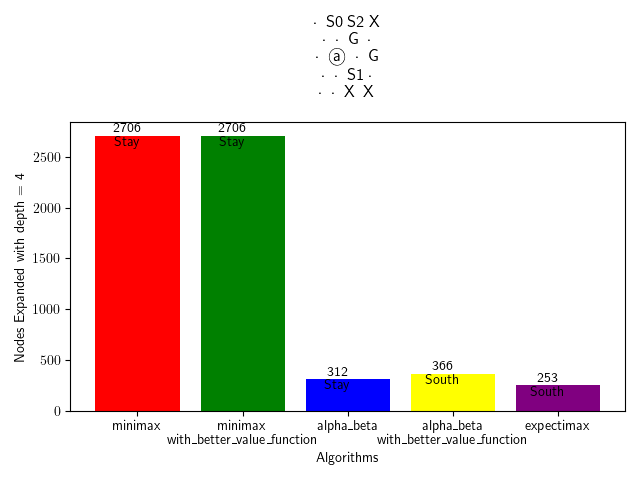
\includegraphics[width=\textwidth]{media/map2023_10_29_13_49_35.png}
    \caption{Map 4}
    \label{fig:image4}
\end{figure}
\vspace{1em}

\paragraph{}
This case shows that better evaluation function does not always mean fewer nodes.

\newpage
\subsection{Fifth Map}




\begin{table}[h]
    \centering
    \begin{tabular}{|c|c|c|c|c|c|}
    \hline
    . & . & L0S & . & . & S2 \\
    \hline
    X & L1S & . & S1 & . & . \\
    \hline
    X & . & . & @ & S0 & X \\
    \hline
    \end{tabular}
    \label{tab:updated_grid}
    \end{table}
        
% Fifth Image
\begin{figure}[h]
    \centering
    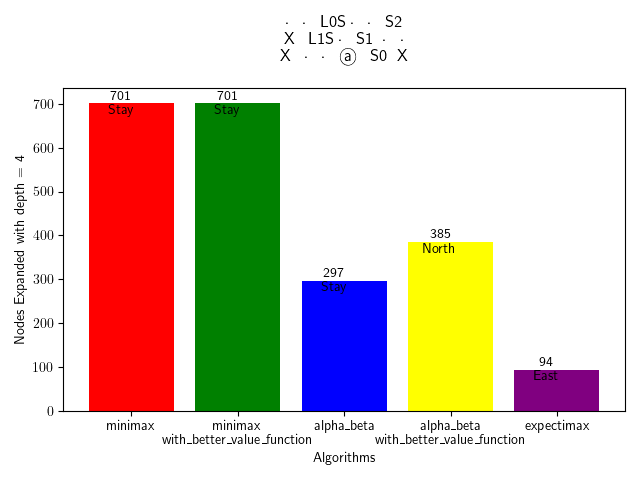
\includegraphics[width=\textwidth]{media/map2023_10_29_13_55_47.png}
    \caption{Map 5}
    \label{fig:image5}
\end{figure}
\vspace{1em}

\paragraph{}
Again, better evaluation function is not the best.

But what makes it very interesting is that \texttt{expectimax} has,
 again, the lowest number of nodes, 
 but also, is the only one to output the optimal action.

\newpage
\section{Discussion}
\subsection{Limitations of High-Level Heuristics}
While the use of high-level heuristics in action ordering 
generally improves performance, 
it is not always fine enough for every case.
As a result, in some cases, the \texttt{BetterValueFunction} 
may not actually result in fewer nodes being expanded 
compared to basic evaluation functions.

\subsection{Use of \texttt{Expectimax}}
Interestingly, the \texttt{Expectimax} algorithm often 
resulted in fewer nodes being expanded 
while also selecting the optimal action. 
This suggests that stochastic models offer benefits in environments 
with high levels of uncertainty.


\subsection{Future Work}
 Recent advancements in adversarial search algorithms have
 started to incorporate machine learning techniques to dynamically 
 adapt the heuristics used for action selection. 
 This represents a potential avenue for further improving 
 the performance of our algorithms.
 
\section{ChatGPT Usage}
The project was made with ChatGPT.
\end{document}
